%!TEX root = main.tex

\section{Folgerungen, Bemerkungen und Beispiele}
    Einleitung KApitel

    \subsection{Zu der Thurston-Norm bei Überlagerungen mit unendlich großer Bettizahl}
        
    \label{verallggruppenring}
    Wie oben bereits vorgeschlagen, kann man nun fragen, welche Anforderungen man an eine Thurston-minimierenden Fläche stellen darf falls $b_1(\ker\phi)=\infty$, also inwieweit lässt sich Lemma~\ref{lem:minS} verallgemeinern? Intuitiv würde man einer unendlich zyklischen Überlagerung schnell die Fähigkeit absprechen, endlich erzeugte Homologiegruppen (über $\ZZ$) zu haben, sind diese Voraussetzungen vielleicht zu restriktiv? Die gute Nachricht ist, dass obiger Beweis nahezu problemlos übertragen werden kann, wenn man nur die endliche Erzeugbarkeit von $\ker\phi$ als $\laurent \QQ t$-Modul fordert. Ob oder wann dies sinnvoll ist soll kurz diskutiert werden, anhand Überlegungen zu nicht endlich erzeugten $\ker\phi$.\\
    Die folgende Proposition kann als Verallgemeinerung der Formel $b_1(\ker\phi)=\Grad\Delta\phi$ aus Corollar~\ref{cor:degreealex} gesehen werden:
    \begin{prop}
    	Falls $H_1(M_\phi)$ endlich erzeugt über dem Gruppenring $\laurent \ZZ t$ ist (dies ist nach Proposition~\ref{prop:alexendlerz} für jede kompakte 3-Mannigfaltigkeit wahr), nicht aber als abelsche Gruppe, so verschwindet die Alexander Norm. Ist umgekehrt $\Delta_{\pi_1(M)}=0$, so folgt dass $b_1(\ker\phi)=\infty$ ist, für alle $\phi\in H^1(M;\ZZ)$
    \end{prop}
    \begin{proof}
    	Die einzige Möglichkeit, dass $H_1(M_\phi;\ZZ)$ über $\laurent \ZZ t$ im Unterschied zu $\ZZ$ endlich erzeugt ist, besteht darin, dass die Familie $\{t_*^kx,k\in\ZZ\}$ in $H_1(M_\phi)$ linear unabhänig über $\ZZ$ ist, wobei $t$ ein Erzeuger der Decktransformationen ist. Also ist $(x)\subset H_1(M_\phi)$ ein freier Anteil des $\laurent \ZZ t$-Moduls. Ohne Einschränkung sieht eine Präsentation von $H_1(M_\phi)$ über dem Gruppenring über $\ZZ$ folgendermaßen aus:
    	\[
    		\begin{xy}
    			\xymatrix@L+3pt{\laurent \ZZ t ^n \ar[r]^{\bigl(\begin{smallmatrix}0&0\\0&X\end{smallmatrix}\bigr)} & \laurent \ZZ t ^n \ar[r] &H_1(M_\phi) \ar[r] &0}
    		\end{xy}
    	\]
    	Somit berechnet sich das Elementarideal zu $E_0(M_\phi)=(\det 0\det X)=(0)$.\\ \todo{Konvention (zur Verallgemeinerung des Grades) ist $||\phi||_A=0 wenn \Delta_\phi=0$}.
    	Andererseits bedeutet gegebenes verschwindendes Alexander Polynom $\Delta_{\pi_1(M)}=0$, dass das Alexander Ideal trivial ist. Das Alexander Ideal aber 
    \end{proof}

    Man sieht also, dass der Fall $b_1(\ker\phi)=\infty$ ein eher triviales Beispiel zur Verifizierung der Abschätzung aus Theorem~\ref{thm:haupttheorem}, also scheinbar uninteressant. Jedoch erschwert das die Situation zur die Berechnung Thurston-Norm, da die untere Schranke entfällt. Nun genug Motivation --- mit der folgenden Proposition soll eine möglichst hohe untere Schranke für das Geschlecht einer Thurston-minimalen zusammenhängenden Fläche angegeben werden:

    \begin{prop}
        Sei $M$ eine 3-Mannigfaltigkeit wie oben und $\phi: \pi_1 \to \ZZ \in H^1(M;\ZZ)$ surjektiv. Weiter sei $H_1(M_\phi)$ ein endlich erzeugter $\laurent \ZZ t$-Modul, wobei $t$ ein Erzeuger der Decktransformationen ist. Nun existiert eine eingebettete orientierbare Fläche $(S,\partial S) \subset (M,\partial M)$, die Folgendes erfüllt:
        \begin{itemize}
            \item $[S]=\phi$
            \item $\chi_-(S) = \thur \phi$
            \item $S$ ist zusammenhängend
            \item Zerlege $H_1(M_\phi;\QQ)\cong \mathcal{F} \oplus \mathcal{T}$ als $\laurent \QQ t$ nach der Klassifikation von endlich erzeugten Moduln über Hauptidealringen in freien und torsions Anteil. Dann ist dies auch eine direkte Summe von $\QQ$-Vektorräumen. Dann soll:
            \[
                b_1(S) \geq  \Rang_{\laurent \QQ t}(H_1(M_\phi;\QQ)) + \dim(H_1(M_\phi;\QQ)/\mathcal F) = \Rang_{\laurent \QQ t} (\mathcal F) + \dim \mathcal T
            \]
            %\item $H_2(S)\cong H_3(M)$
        \end{itemize}
    \end{prop} 
    \begin{bem}
        Die Aussage ist analog zu Lemma~\ref{lem:minS}, wobei die Aussagen 
    \end{bem}
    \begin{proof}
        Man wähle unter den eingebetteten Fläche welche die ersten beiden Eigenschaften erfüllen, also Thurston-Norm-minimierend sind, eine Fläche aus deren Anzahl an Zusammenhangskomponenten möglichst gering ist. Mit der gleichen Konstruktion des Graphen wie im Beweis des Lemmas~\ref{lem:minS} argumentiert man, dass $S$ zusammenhängend ist.\\
        Da $\mathcal F \subset H_1(M_\phi;\QQ)$ als Moduln über dem Ring der rationalen Laurentpolynome endlich erzeugt sind, erzeugt ein kompakter Teilraum der Überlagerung $\mathcal F$ als Gruppenring Modul. Mit diesem Argument folgt wie im Beweis des Lemmas, dass $b_1(S)\geq \Rang(\mathcal F)$. Da $\mathcal T \subset H_1(M_\phi;\QQ)$ nun endlich erzeugt als Vektorraum ist, folgt mit dem Kompaktheitsargument, dass auch hier $S$ diesen Vektorraum erzeugt, also $b_1(S)\geq \dim \mathcal T$. $\mathcal F$ und $\mathcal T$ sind invariant bezüglich der Decktransformationen (sie sind direkte Summanden über dem Gruppenring). Das erlaubt uns Repräsentanten $f_1,\cdots,f_{\Rang(\mathcal F)},t_1,\cdots,t_{\dim\mathcal T}$ zu wählen, die Basis eines $\Rang(\mathcal F)+\dim\mathcal T$-dimensionalen $\QQ$-Vektorraums sind und die $f_i$ erzeugen $\mathcal F$ als Gruppenringmodul. Offensichtlich ist dieser Raum \emph{nicht} $t_*$-invariant, genauer: dieser Vektorraum ist eine direkte Summe aus einem $t_*$-invarianten und einem nicht-$t_*$-invarianten Raum. Allerdings folgt nun aus den obigen Überlegungen, dass die $f_i$ so gewählt werden können, dass die Inklusion $S\into M_\phi$ auf der ersten Homologie mit $\QQ$-Koeffizienten, eine lineare Abbildung induziert dessen Bild $\langle f_1,\cdots,f_{\Rang(\mathcal F)},t_1,\cdots,t_{\dim\mathcal T} \rangle$ enthält.
    \end{proof}

    Leider sieht man, dass Lemma~\ref{lem:minS} nicht direktes Corollar dieser Proposition ist, da im letzten Beweis $b_2(S)=b_3(M)$ nicht gezeigt werden kann. Ist $b_2(S)=0$ (da $S$ zusammenhängend ist $b_2 \in \{0,1\}$), so folgt $\partial S \neq \emptyset$ und somit $\partial M \neq \emptyset$, also Gleichheit $b_2(S)=b_3(M)$. Ist allerdings $b_1(S)=1$, also $S$ eine geschlossene Fläche, so folgt \emph{nicht} zwangsweise, dass $M$ geschlossen ist:
    \begin{bsp}
     Man betrachte etwa den 3-dimensionalen Torus $M=T=S^1\times S^1 \times S^1$ mit $H_1(M)=\ZZ^3 \cong \Hom(H_1(M),\ZZ) \cong H^1(M;\ZZ)$ nach dem universellen Koeffiziententheorem und der Produktverträglichkeit der Fundamentalgruppe, so wie Hurewicz. Nun betrachte man eine Fläche die dual zu einem der kanonischen Erzeuger der Fundamentalgruppe ist, am einfachsten wäre zum Beispiel $S=* \times S^1 \times S^1$ mit der zugehörigen durch Aufschneiden und Verkleben -gewonnenen Überlagerung $\RR \times S^1 \times S^1$ die homologisch endlich erzeugt ist. Sicher ist es möglich einen glatt eingebetteten $2$-Volltorus $U\cong S^1\times D$ aus dem Komplement von der betrachteten Fläche $S$ zu finden. Betrachtet man nun die Mannigfaltigkeit $N=M - \mathring U$, so erhält man eine glatte orientierbare Mannigfaltigkeit mit Rand $(N,\partial N)= (M- \mathring U, \partial U)$, die auch sonst alle Voraussetzungen der vorhergehenden Proposition erfüllt. Da $U$ zu $S$ durchschnittsleer gewählt wurde, ist $[S]$ sicherlich eine nicht-triviale Homologieklasse in $H_2(N,\partial N;\ZZ)$. Nun ist die durch Aufschneiden und Verkleben an $S$ - gewonnene Überlagerung über dem Gruppenring endlich erzeugt, aber $b_2(S)=1 \neq 0 = b_3(N)$.
    
    \end{bsp}

    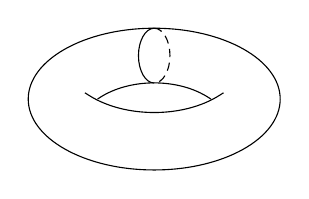
\begin{tikzpicture}
    %Torus
    \draw (0,0) ellipse (1.6 and .9);
    %Hole
    \begin{scope}[scale=.8]
    \path[rounded corners=24pt] (-.9,0)--(0,.6)--(.9,0) (-.9,0)--(0,-.56)--(.9,0);
    \draw[rounded corners=28pt] (-1.1,.1)--(0,-.6)--(1.1,.1);
    \draw[rounded corners=24pt] (-.9,0)--(0,.6)--(.9,0);
    \end{scope}
    %Cut 1
   % \draw[densely dashed] (0,-.9) arc (270:90:.2 and .365);
   % \draw (0,-.9) arc (-90:90:.2 and .365);
    %Cut 2
    \draw (0,.9) arc (90:270:.2 and .348);
    \draw[densely dashed] (0,.9) arc (90:-90:.2 and .348);
    \end{tikzpicture}

    \subsection{Faserungen}

    In diesem Abschnitt, wollen wir uns mit Faserungen über dem Kreis beschäftigen.
        
    \begin{bsp}
    	Sei $M$ eine Faserung $M\to S^1$ über dem Kreis ist, also es gibt einen Diffeomorphismus einer zusammenhängenden Fläche $\varphi: S \times 0 \to S\times 1$, so dass folgendes Diagramm kommutiert:
    			\todo{f mittig}
    	\[
    		\begin{xy}
    			\xymatrix{M \ar[r]^f \ar[d] &I/\partial I = S^1 \\
    					S\times I /\varphi \ar[ru]_{p_2}}
    		\end{xy}
    	\]
    	In diesem Fall definiert die Homotopieklasse der Faserung $M \to S^1$ eine eindeutige Kohomologieklasse $\phi\in H^1(M;\ZZ)$. Die Überlagerung $M_\phi$ kann wieder entweder als Rückziehung von $\RR \to S^1$ oder durch Aufschneiden an $S$ gewonnen werden --- in beiden Fällen ist leicht ersichtlich, dass $M_\phi \cong S \times \RR$ ist (für das Aufschneiden an $S$, benötigt man das $[S]=\phi$, dies gilt aber da jedes Urbild von einem Punkt unter $f$ diffeomorph zur Fläche ist, insbesondere die der regulären Werte, die nach Sard existieren). Also hat $M_\phi$ den Homotopietyp der Fläche, dementsprechend berechnen sich die Homotopieinvarianten von $M_\phi$. \todo{Erwähnen, dass ker(phi) immer den Kern als Abbildung auf der FG bedeutet} Insbesondere ergibt sich $b_1(\ker\phi) =b_1(M_\phi)= b_1(S)$, wodurch sich mit Lemma~\ref{lem:minS} ergibt (da $b_0(S)=1$), dass die duale Fläche mit Gleichheit der ersten Bettizahlen gewählt werden kann. Da dies die einzige Ungleichung ist, die in dem Theorem verwendet wird, folgt also schon Gleichheit der Normen $||\phi||_A = ||\phi||_T$, falls $b_1(M)>1$ und $||\phi||_A = ||\phi||_T+1+b_3(M)$ sonst. Aufgrund der exakten Sequenz:
    	\[
    		0 \to \ker\phi \to \pi_1(M) \to \ZZ \to 0
    	\]
    	folgt auch das die Fundamentalgruppe von $M$ im Falle einer Faserung endlich erzeugt ist. Falls $M$ nun zusätzlich noch ein Knotenkomplement eines Knotens $K$ ist, gilt $\ker\phi = [\pi_1(M),\pi_1(M)]$. Also beweisen diese Überlegungen, dass die Kommutatorunteruntergruppe einer Knotengruppe isomorph zu der Fundamentalgruppe einer Seifertfläche des Knotengeschlechts ist, siehe zum Beispiel Theorem 4.6 in~\cite{Burde.2003}.\\
        Es stellt sich die Frage, in wie weit eine Faserung eindeutig ist. Beispielsweise ist im Falle eines Vektorbündels über einem zusammenhängendem Raum, die Dimension eindeutig. Falls aber $b_1(M)>1$ ist und $\phi,\psi \in H^1(M;\ZZ)$ Repräsentanten in $[M,S^1]$ haben die Faserungen sind, folgt dann etwa: $||\phi||_T=||\psi||_T$? Existieren Diffeomorphismen zwischen Abbildungstori zu Flächen verschiedenen Geschlechts? Tatsächlich sind die Faserungen nicht eindeutig siehe Beispiel~\ref{ex:fiberedfaces}.\\
    	Möchte man dennoch das Alexander Polynom $\Delta_f=\Delta_\phi$ einer Faserung $f$ berechnen \todo{gilt das für Betti>1?}(falls $b_1(M)=1$ ist $\Delta_f=\Delta_M$), schließlich benutzt diese Invariante ja noch Informationen über die Deckgruppe, genügt es nach Lemma~\ref{lem:charPol}, die lineare Form von Vektorräumen $t_* \in \Aut(H_1(M_\phi;\QQ))$ zu berechnen. Aber da der Erzeuger $t$ der Decktransformationen folgendem kommutativen Diagramm genügen muss:
    	\begin{equation*}
     		    	\begin{xy}
    			\xymatrix{
    				&S \ar[d]^{\simeq} \ar[dl] \ar[rr]_\cong && S \ar[d]^{\simeq}\ar[dr]& \\
    				M_\phi \ar[ddrr] \ar[r]^\cong&S \times \RR \ar[rr]^{\hat t}_\cong \ar[dr] && S\times \RR \ar[dl] \ar[r]^\cong&M_\phi \ar[ddll]\\
    				&&S\times I / \varphi \ar[d]^\cong&&\\
                    &&M&&}
    		\end{xy}
    	\end{equation*}
    	und andererseits $t_*$ von einem Lift der zur Faserung dualen Schleife induziert wird, muss in jedem Fall gelten: $t_* = \hat t_* = \varphi$ unter gegebenen Identifikationen mit $S$. Also berechnet sich das Alexander Polynom $\Delta_f$ zu dem charakteristischen Polynom der Abbildung $\varphi_*:H_1(S;\QQ)\to H_1(S;\QQ)$, wobei die Koeffizienten entsprechend in $\ZZ$ gewählt werden, so dass es größter gemeinsamer Teiler des entsprechend zurückgezogenen Ideals unter der Lokalisierung $\ZZ \to \ZZ^{-1}\ZZ=\QQ$ ist. Alternativ lässt sich das Alexander Polynom einer Faserung $[f]$ auch berechnen, indem man die Aufschneide und Verklebe Konstruktion für unendlich zyklische Überlagerungen verwendet. Dort stellt man fest, dass jede aufgeschnittene Kopie den Homotpietyp der Fläche hat und dass bei Verkleben je zweier Kopien, die Relationen von $\varphi_*$. Dies liefert eine Präsentation als Gruppenring Modul, wobei man feststellt, dass alle diese Relationen äquivalent sind, da die Decktransformationen die Einheiten des Gruppenrings sind. Man beachte, dass dies ein Spezialfall der "`Aufschneiden und Verkleben"'-Konstruktion ist, da $M$ selber durch Verkleben entsteht aus $S\times I$. So erhält man also eine $n$-blättrige Überlagerung von $M$, indem man $n$ Kopien von $S\times I$ anhand $\phi$ aneinander klebt.\\
        Dies liefert die Möglichkeit in diesem Beispiel für $b_1(M)=1$ das Theorem zu verifizieren (nicht wie oben zu nutzen), indem man berechnet: \todo{Orientierbarkeit und}
        \[
            ||\phi||_A=\Grad(\Delta_\phi)=\Grad (\Delta_f) = \Grad \det (\varphi_*-tI) = g(S) = \chi_-(S) +2 = ||\phi||_T+2
        \]

        Im Falle der trivialen Bündel $D^2\times S^1$ oder $S^2\times S^1$ stimmt die zyklische Überlagerung mit der universellen überein und man erhält jeweils $\Delta_\phi =1$ für $\phi$ einen Erzeuger der ersten Homologie. Da die Erzeuger für $H_2(D^2 \times S^1, \partial)\cong \ZZ$ und $H_2(S^2\times S^1) \cong \ZZ$ sich mit Poincaré Dualität als $[D^2,\partial D^2]$ beziehungsweise $[S^2]$ herausstellen, verschwindet auch die Thurston-Norm. In diesem Fall gilt also keine Gleichheit in Theorem~ref. 

    \end{bsp}

    \begin{bsp}
        Handelt es sich bei $M$ um eine Faserung $M\to S^1$ mit $b_1(M)=1$ oder ist $b_1(M)>1$ und jede Kohomologieklasse repräsentiert durch eine Faserung, so berechnet sich die Thurston-Norm nach Theorem~\ref{thm:haupttheorem} bereits vollständig durch die Fundamentalgruppe, siehe Kapitel~\ref{sec:algebra}.
    \end{bsp}


    \begin{bsp}
    \label{ex:fiberedfaces}
        Eine wichtige Anwendung der Thurston Norm und dieser Abschätzung besteht in den sogenannten \textit{fibered faces}, die im Folgenden als gefaserte Seiten bezeichnet werden. Bisher wurden bereits Kohomologieklassen $\phi \in H^1(M;\ZZ)$ betrachtet, mit einer korrespondenten Abbildung $M \to S^1$ die eine Faserung darstellt. Bei solchen herrscht Gleichheit im Theorem (siehe ref). Diese Klassen werden auch als \textit{gefasert} bezeichnet. Tatsächlich stellt Thurston in \cite{Thurston.1986} fest, dass Informationen über diese Eigenschaft durch die Thurston-Norm festgestellt werden. Wie in Bemerkung~\ref{rem:extendingthurston} gezeigt, lässt sich die Thurston-Norm durch Erweiterung der Skalare (tensorieren mit $\RR$), fortsetzen. Thurston hat in \cite{Thurston.1986} außerdem gezeigt, dass der Einheitsball dieser Norm auf $H^1(M;\RR)$ ein beschränktes konvexes Polytop ist, also die konvexe Hülle einer endlichen Anzahl an Elementen. Eine berandende Seite dieses Polytops, nennt man gefaserte Seite, falls alle Elemente $\phi \in H^1(M;\ZZ)$ die auf einem vom Ursprung ausgehendem Strahl liegen der das Innere der Seite trifft, gefasert sind. Anders gesagt ist eine Seite gefasert, genau dann wenn jedes $\phi \in H^1(M;\ZZ)$, das in einem Kegel mit dem Inneren der Seite als Grundfläche und dem Ursprung als Spitze, gefasert ist. Natürlich ist das Polytop symmetrisch ($||-\phi||_T=||\phi||_T$) und die gefaserten Seiten treten auch in Paaren auf (eine Faserung $M \to S^1$ liefert mit einer orientierungsumkehrenden Reflektion $\tau$ das Inverse $M \to S^1 \stackrel \tau \to S^1$). Man sagt, gefaserte Klassen $\phi,\psi$ liegen in \textit{wirklich verschiedenen} gefaserten Kegeln, falls diese bis auf Symmetrie verschieden sind. 
    \end{bsp}

    \begin{bem}
        Zwei Normen zu abzuschätzen ist gleichbedeutend eine Inklusionsbeziehung ihrer Einheitsbälle festzustellen.
    \end{bem}

    \subsection{Knoten und Verschlingungen}
    \label{sec:links}
    \begin{bsp}[Verschlingungen]
    \label{ex:links}
        Thurston liefert einige Beispiele in Form von Verschlingungskomplementen, als er sein Ergebnis über die Existenz "`seiner"' Norm und ihren Einheitsball veröffentlicht \cite{Thurston.1986}. Eine Verschlingung bezeichnet eine gemeinsame disjunkte Einbettung von mehreren Knoten, also eine glatte Einbettung $L: \sqcup_{i=1}^m S^1 \to S^3$. Als $M_L$ bezeichnen wir wieder die kompakte 3-Mannigfaltigkeit, die aus Entfernen einer offenen Tubenumgebung hervorgeht. Wählt man auf $\sqcup S^1$ die Standardorientierung, erhält man wie im Fall eines Knotenkomplements, kanonische Erzeuger von $H^1(M_L)$, nämlich durch folgende Überlegungen: eine Orientierung einer Komponente liefert (nach festgelegter Konvention) einen orientierten Meridian, das ist eine Schleife die in $M_L\stackrel \simeq \into M - \im(L)$ homotop zu einer Einbettung einer Einheitssphäre einer Faser unter einer Tubenabbildung ist (es lässt sich in einem trivialen Bündel leicht von einer Einheitssphäre sprechen). Diese liefern kanonische Erzeuger der ersten Homologie $H_1(M_L) \cong \ZZ^m$ die kanonische Basis des Dualraums $l_1,\cdots,l_m \in H^1(M_L)\cong H_1(M_L)$ geht also kanonisch aus den Komponenten der Verschlingung $L_1,\cdots,L_m$ hervor. Außerdem liefert dies eine kanonische Identifikation mit dem Laurentring $\ZZ[ab(G)]=\ZZ[l_1^{\pm 1},\cdots,l_m^{\pm 1}]$ (analog wie im Knotenfall). Um also beispielsweise den Einheitsball der Thurston-Norm zu beschreiben, lassen sich ebenfalls (per Konvention) die Koordinaten $l_i=l_i \tensor 1 \in H^1(M)\tensor \RR = H^1(M;\RR)$ verwenden (diese Konvention nutzt natürlich, dass die eben beschriebene Konstruktion kanonisch ist).\\

    \end{bsp}
        \todo{siehe Kommentar Thurston, dass keine Komponente Scheibe beranden oder Kreisring beranden soll}
        \texttt{Berechnung der Einheitsbälle einiger Verschlingungen}
        \texttt{Knoten}
        Im Fall, dass der Link nur aus einer Komponente besteht --- es sich also um einen Knoten handelt --- ist $H^1(M;\RR)\cong \RR$. Sei $\phi$ ein Erzeuger der ganzzahligen Kohomologie, dann ist $\phi$ dual zu der Seifertfläche und jede duale Fläche ist eine Seifertfläche. Somit ist (solange nicht vom Unknoten geredet wird) wie oben erwähnt $||\phi||_T=2g(L)+1$. Also in der ist die abgeschlossene Einheitskugel der Thurston-Norm gegeben durch:
        \begin{eqnarray*}
            H^1(M;\RR) &\cong & \RR \\
            {[- \frac{1}{2g(L)+1} \phi,\frac 1 {2g(L)+1} \phi]} & = \bar B_{||\cdot||_T}=& {[- \frac 1 {2g(L)+1}, \frac 1 {2g(L)+1}]}
        \end{eqnarray*}
        wobei dann entsprechend für die duale Thurston-Norm $||\cdot||_T^* : H_1(M;\RR)\to \RR$ (mit Ausnutzung der Symmetrie) folgt:
        \[
            \bar B_{||\cdot||_T^*} = \{\alpha \in H_1(M;\RR), \frac{1}{2g(L)+1}\phi (\alpha)\leq 1\} = {[-(2g(L)+1)\hat \alpha, (2g(L)+1) \hat \alpha]}
        \]
        Hier wird unter dem natürlichen Isomorphismus $H_1((M;\RR) \cong H_1(M;\RR)^{**} \cong \Hom(H^1(M;\RR),\RR)$ die duale Thurston-Norm über der ersten Homologie aufgefasst und $\hat \alpha$ als Erzeuger der ganzzahligen Homologie, genauer gesagt, der Homologieklasse --- nach obiger Konvention --- \emph{des} Meridians (also gilt $\phi(\hat \alpha)=1$). 
        \begin{bem}
            Da dies keine Arbeit über die Eulercharakteristik einer Fläche ist, möge der Leser in den folgenden Beispielen zur Berechnung der Eulercharakteristik dualer Flächen (hier: Seifertflächen) seine liebste Formel verwenden.
        \end{bem}
        \texttt{Hopf Verschlingung}
        \begin{wrapfigure}{r}{0.4\textwidth}
            \centering
            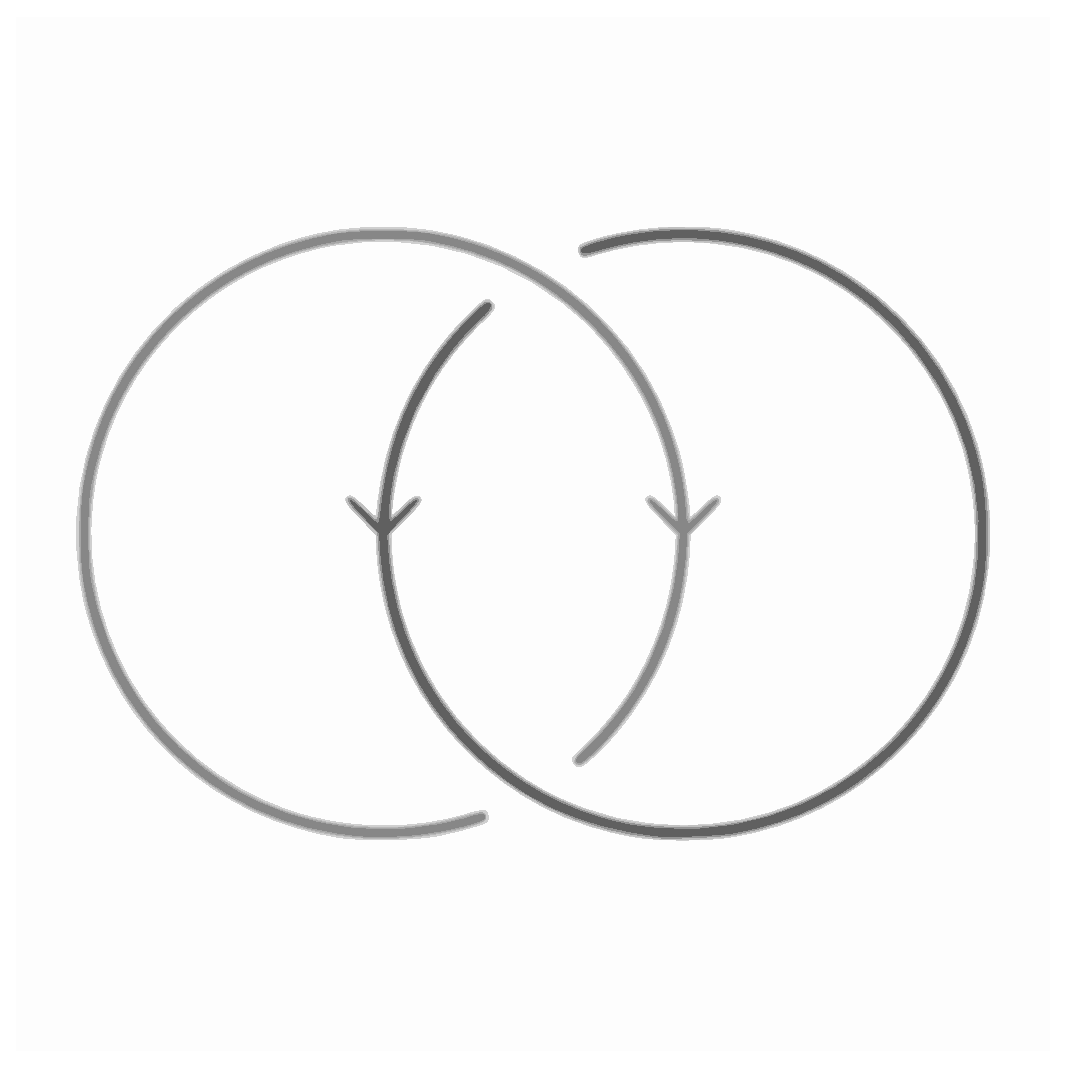
\includegraphics[width= 0.3\textwidth]{hopf}
            \caption{Die Hopf Verschlingung}
            \label{fig:hopf}
        \end{wrapfigure}
        Das trivialste nicht-triviale Beispiel einer Verschlingung mit mehreren Komponenten ist der Hopf Link. Er besteht aus zwei ineinander verschlungenen Unknoten, $L_1, L_2$. Betrachtet man nun zwei Scheiben und verklebt diese mit zwei umgekehrt verdrehten Bändern, so erhält man die Hopf Verschlingung als Rand. Äquivalent möge man sich einen Kreisring $S^1 \times I$ nehmen, der zweifach verdreht ist und beobachtet, dass dieser eine Seifertfläche $S$ darstellt. Das Geschlecht dieser Seifertfläche ist $0$, da es sich um eine Sphäre handelt, aus der zwei offene Scheiben entnommen wurde. Andersherum erhält man durch Ankleben zweier Scheiben die Eulercharakteristik $\chi_-(S)=0$. Da zu gegebener Orientierung $[S] = \epsilon_1 [l_1]+ \epsilon_2 [l_2]$ ($\epsilon_i \in \{\pm 1\}$) verschwindet mit der Subbadditivität die Thurston-Norm auf dem Vektorraum $H^1(M;\RR)$, also ist die Einheitskugel nicht kompakt, sondern der gesamte Raum. Geht man jedoch zur dualen Norm über, erhält man wieder ein kompaktes Polytop mit ganzzahligen Eckpunkten: 
        \[
              \bar B_{||\cdot||_T^*}= \{\alpha \in H_1(M;\RR)| \sup_{\{\phi \in H^1(M;\RR)\}} \phi(\alpha)\leq 1\}=0
        \] 
        \texttt{Whitehead Verschlingung}
        Die Whitehead Verschlingung ist ein Link der aus zwei Komponenten $L_1,L_2$ besteht. Offensichtlich berandet jede Komponente $L_i$ in $M_{L_i}$ eine Scheibe, die sich in $M_L$ auf eine Kreisscheibe mit zwei entnommenen offenen Scheiben einrschänkt (an den Stellen, an dem die offene Tubenumgebung des anderen Knotens die Scheibe durchdringt). Bei diesen Repräsentanten für $l_1$ beziehungsweise $l_2$ berechnet sich die Eulercharakteristik zu $-1$, also gilt $||\pm l_i||_T\leq 1$, offensichtlich gilt aber Gleichheit. (Nun ist aber in diesem Fall die Thurston-Norm eine tatsächliche Norm, ) Genauso offensichtlch gilt $||l_1+l_2||_T>0$: die Verschlingungszahl des Whitehead Links ist offensichtlich $0$ (dies sieht man indem man eine Projektion betrachtet in dem die eine Komponente der Unknoten ist), jedoch haben die Randkomponenten jeder Einbettung eines Kreisring $S^1\times I \into S^3$ Verschlingungszahl $\neq 0$ oder sind trivial (durch einen Äquator zu trennen). Also folgt $2 \leq ||l_1+l_2||_T \leq ||l_1||_T+||l_2||_T =2$ für eine Seifertfläche. Diese ist sogar einfach durch die Seifert-Konstruktion zu erhalten. Folglich:
        \begin{align*}
            ||l_1+l_2||_T =||-(l_1+l_2)||_T &\stackrel * = ||-l_1+l_2||_T = ||l_1-l_2||_T \\
            &=2
        \end{align*}
        wobei die ausgezeichnete Gleichung gilt, da $||-l_1+-l_2||_T\not \in \{0,1\}$ aus obigen Gründen.
        \emph{Behauptung:} Die Thurston-Norm Einheitskugel und ihr Duales sind die Folgenden:\\
        \begin{figure}[H]
        \centering
        \begin{subfigure}[l]{0.4\textwidth}
                \begin{tikzpicture}
            % Axis
            \draw[->] (-3,0)--(3,0) node[below] {$l_1$};
            \draw[->] (0,-3)--(0,3) node[left] {$l_2$};
        
            \draw[] (0,2)--(1,1);
            \draw[] (1,1)--(2,0);
            \draw[] (2,0)--(0,-2);
            \draw[] (0,-2)--(-2,0);
            \draw (-2,0)--(0,2);
        
            \node[below] at (2,0) {$l_2$};
            \node[above right] at (1,1) {$\frac {l_1+l_2}2$};
           % \filldraw[black] (1,1) circle (2pt) node[above right,black] {$\frac {l_1+l_2}2$};
            \foreach \Point in {(0,2), (1,1), (2,0), (0,-2), (-2,0), (0,2), (1,-1), (-1,-1),(-1,1)}{
            \node at \Point {\textbullet};
            }
        
            \end{tikzpicture}
                \caption{$\thurball$}
        
        
        \end{subfigure}    
        \hfill
    \begin{subfigure}[r]{0.4\textwidth}
              \begin{tikzpicture}
        % Axis
        \draw[->] (-3,0)--(3,0) node[below] {$L_1$};
        \draw[->] (0,-3)--(0,3) node[left] {$L_2$};

        \draw (-2, -2) --(-2, 0) --(-2, 2) --(0 ,2) --(2 ,2)--(2 ,0)--(2 ,-2) --(0 ,-2) --(-2,-2) ; 
        \foreach \Point in{(-2, -2) ,(-2, 0) ,(-2, 2) ,(0 ,-2) ,(0 ,2) ,(2 ,-2) ,(2 ,0) ,(2 ,2)}{
        \node at \Point {\textbullet};
        }
        \end{tikzpicture}
    \caption{$\dualthurball$}

    \end{subfigure}
    \caption{Einheitskugeln der Whitehead Verschlingung in $H^1(M;\RR)$ und $H_1(M;\RR)$}
    \end{figure}
    Die $8$ berechneten Punkte liegen auf dem Rand von $\thurball$ (die Norm ist stetig), einer konvexen Teilmenge. Es ist eine leichte Übung, dass jede konvexe Teilmenge zweier nächster Punkte im Rand dieser konvexen Teilmenge enthalten sein muss. Aufgrund der Monotonie folgt die Behauptung für die Einheitskugel. Für die duale Norm, berechnet man entweder $8$ verschiedene Randpunkte, oder beobachtet für jedes $\alpha \in H_1(M;\RR)$ auf welchem Elementen (eine Gerade) $\phi \in H^1(M_L;\RR)$ das Supremum $\phi \alpha$ angenommen wird und sieht direkt das Ergebnis.
    \texttt{Borromäische Ringe}
    Seien $L=L_1 + L_2 + L_3$ die Borromäischen Ringe. Offensichtlich hat jede duale Fläche zu $l_i$, die Komponente $L_i$ als Rand, (sonst wäre der Meridian aufgrund eines Schnittzahlen Argumentes im Kern von $l_i$). Folglich hat also jede Fläche dual zu $l_i$ mindestens 3 Randkomponenten. Da eine Sphäre mit 3 (also eine abgeschlossene Scheibe mit 2 Durchlöcherungen) entnommenen offenen Scheiben, wobei die eine Randkomponente aufgespannt wird von der entnommenen Komponente $\nu(L_i)$, bereits dual zu $l_i$ ist gilt wieder $\thur {\pm l_i}=1$ für jedes $i$. Ähnlich wie beim letzten Beispiel der Whitehead Verschlingungen, möchten wir nun --- in Dimension 3 --- die berandenden Seiten der Einheitskugel durch Berechnung einiger Punkte feststellen und sie dadurch feststellen. Als nächstes betrachte man $l=l_1+l_2+l_3$, also ist eine Geschlecht-minimale Seifertfläche gesucht. Allerdings lässt sich die Thurston-Norm von $l$ auch mit geschickter Argumentation begründen. Zunächst gilt für die Halbnorm $\thur l \leq \thur {l_1} + \thur {l_2} + \thur{l_3}=3 \implies \thur l \in \{1,3\}$. Außerdem gilt für alle $\phi,\psi \in \{\pm l_1 \pm l_2 \pm l_3\}: \thur \phi = \thur \psi$, da duale Flächen unter Veränderung der Orientierung einzelner Komponenten in $1-1$ Beziehung stehen, also ist das Geschlecht $g(L)$ der Borromäischen Ringe unabhängig von der Orientierung. Durch Bestimmung der Werte an $\pm l_i$ folgt schon, dass jede konxeve Menge die konvexe Hülle der Einheitspunkte $\pm l_i$ enthalten muss --- den Einheits-Oktaeder. Also ist $\thur l \neq 1$, sonst würden zwei benachbarte der obigen Randpunkte 

\begin{figure}
\centering
    \begin{subfigure}{0.4\textwidth}
    
        \tdplotsetmaincoords{70}{110}        
        \begin{tikzpicture}[tdplot_main_coords]

        \draw[dashed] (-2,0,0) -- (2,0,0) ;
        \draw[dashed] (0,-2,0) -- (0,2,0) ;
        \draw[dashed] (0,0,-2) -- (0,0,2); 
        \draw[->] (2,0,0) -- (3,0,0) node[anchor=north east]{$l_1$};
        \draw[->] (0,2,0) -- (0,3,0) node[anchor=north west]{$l_2$};
        \draw[->] (0,0,2) -- (0,0,3) node[anchor=south]{$l_3$};
    
    
        \foreach \x in {2,-2}{
                \node at (\x  ,0,0) {\textbullet};
                \node at (0,\x ,0) {\textbullet};
                \node at (0,0,\x ) {\textbullet};
                \draw (\x,0,0)--(0,\x,0);
                \draw (\x,0,0) -- (0,0,\x);
                \draw (\x,0,0)--(0,-\x,0);
                \draw (\x,0,0) -- (0,0,-\x);
                \draw (0,\x,0) -- (0,0,\x);
                \draw (0,\x,0) -- (0,0,-\x);
                }
            \draw [fill,opacity=0.3] (2,0,0) -- (0,2,0) -- (0,0,2) -- cycle;
         %   \draw[thick] (2/3-0.3,2/3,2/3) -- (2/3+0.3,2/3,2/3);
            \draw[thick] (2/3,2/3-0.2,2/3) -- (2/3,2/3+0.2,2/3);
            \draw[thick] (2/3,2/3,2/3-0.2) -- (2/3,2/3,2/3+0.2);
            \node[above] at (2/3+0.2,2/3,2/3+0.2) {$l/3$};
        \end{tikzpicture}
        \caption{$\thurball$}
    \end{subfigure}
    \hfill
    \begin{subfigure}[r]{0.4\textwidth}
    
        \tdplotsetmaincoords{70}{110}
        \begin{tikzpicture}[tdplot_main_coords]

        \draw[dashed] (-2,0,0) -- (2,0,0) ;
        \draw[dashed] (0,-2,0) -- (0,2,0) ;
        \draw[dashed] (0,0,-2) -- (0,0,2); 
        \draw[->] (2,0,0) -- (3,0,0) node[anchor=north east]{$l_1$};
        \draw[->] (0,2,0) -- (0,3,0) node[anchor=north west]{$l_2$};
        \draw[->] (0,0,2) -- (0,0,3) node[anchor=south]{$l_3$};
    
        \foreach \x in {2,-2}{
                \node at (\x  ,0,0) {\textbullet};
                \node at (0,\x ,0) {\textbullet};
                \node at (0,0,\x ) {\textbullet};
                }
        \foreach \x in {2,-2}{
            \foreach \y in {2,-2}{
            \foreach \z in {2,-2}{
            \draw (\x,\y,\z) -- (\x,\y,-\z);
            \draw (\x,\y,\z) -- (-\x,\y,\z);
            \draw (\x,\y,\z) -- (\x,-\y,\z);
            }
            }
        }
        \end{tikzpicture}
        \caption{$\dualthurball$}
    \end{subfigure}
    \caption{Die Einheitskugeln der Borromäischen Ringe}
\end{figure}
    \begin{bsp}
        Eine (Halb-)Norm auf einem Vektorraum, liefert stets eine (Halb-)Norm auf seinem Dualraum. Diese ist für einen Vektorraum $(V,|\cdot|)$ auf dem Dualraum $(V^*,||\cdot||)$ definiert durch:
        \[
             ||\alpha||= \sup_{\{v\in V, |v|=1\}} |\alpha v|
         \] 
         Entsprechend übertragen sich die Alexander und Thurston Norm auf die erste (relative) Homologie und die zweite (relative) Kohomologie der 3-Mannigfaltigkeit. 
    \end{bsp}